\subsection{Filterspezifikation}

Beim zu realisierenden Stubfilter handelt es sich um ein Tiefpass-Filter 5. Ordnung, mit einer Grenzfrequenz (Passband) $f_C = 0.8GHz $ und einer Bezugsfrequenz $f_{\frac{\lambda}{4}} = 2GHz$. Die Bezugsfrequenz $f_{\frac{\lambda}{4}}$ definiert die Länge l der gleich langen Leitungsstücke uns ist folglich:

\begin{equation*}
l = \frac{\lambda}{4} = \frac{c}{4 \cdot f} = \frac{300\cdot 10^6 \lbrack\frac{m}{s}\rbrack}{4 \cdot 2 \lbrack GHz \rbrack} =37.5 \lbrack mm \rbrack
\end{equation*}

Das Stubfilter wird von einem Prototypfilter (Tiefpass 5. Ordnung) 
mit den Elementwerte $g_0$ bis $g_6$ abgeleitet.

\begin{figure}[h!]
\centering
 	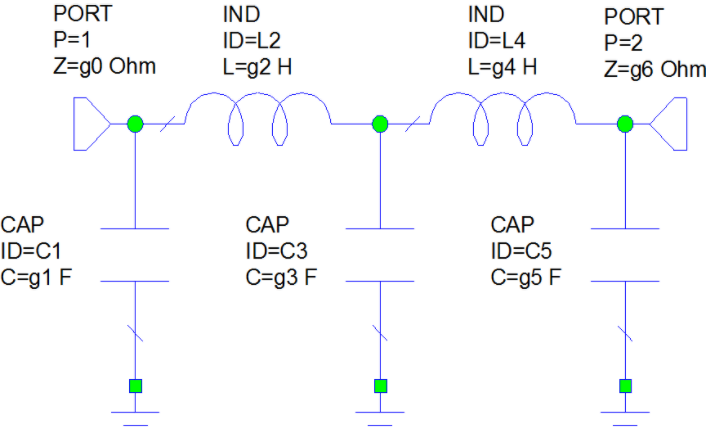
\includegraphics[width=\imagewidth]{images/Topologie_Prototyp.png}
 	\caption{Topologie des Prototypfilters}
 	\label{fig:Topologie_Prototyp.png}
\end{figure}

\begin{mdframed}
    \begin{align*} 
        g_0 &= 1 \\ 
        g_1 &= 0.973 \\ 
        g_2 &= 1.372 \\ 
        g_3 &= 1.803 \\ 
        g_4 &= 1.372 \\ 
        g_5 &= 0.973 \\ 
        g_6 &= 1 \\ 
    \end{align*} 
\end{mdframed}

Durch eine Simulation in Mirowave Office (MWO) kann gezeigt werden, dass es sich beim Prototypfilter um ein Chebyshev Filter des Typs 1 handelt, weil das Filter im Passband einen Equirippel und im Stopband keinen Rippel aufweist. 

Die Übersichtsdarstellung der Eingügedämpfung S21 (Abb. \ref{fig:Ovw_Prototyp}) zeigt, dass das Filter keinen Stopbandrippel aufweist.

\begin{figure}[h!]
    \centering
 	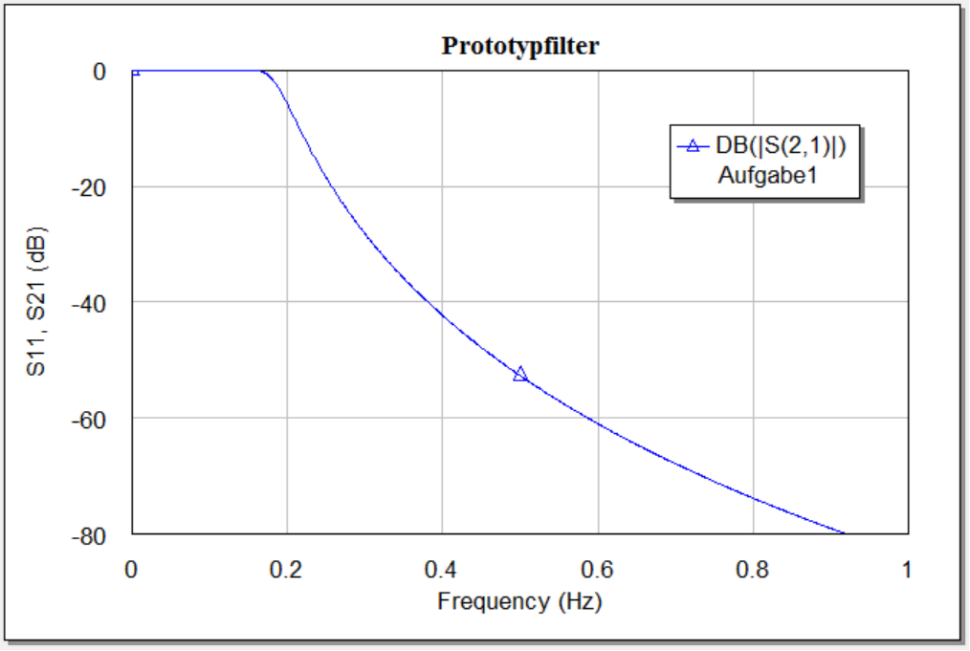
\includegraphics[width=\imagewidth]{images/Ovw_Prototyp.png}
 	\caption{Übersichtsdarstellung des Prototypfilters}
 	\label{fig:Ovw_Prototyp}
\end{figure}

Erst die Detailanssicht der  Einfügedämpfung  S21  in  Abb. \ref{fig:graph-LC}
zeigt, dass das Prototypfilter im  Passband auch noch einen kleinen Equirippel
aufweist. Ausserdem zeigt  sich  aus der Detailansicht, dass das Filter wie er
erwartete eine Grenzfrequenz von $\omega_C = 1$ aufweist.

\begin{mdframed}
    \begin{equation*} 
        \begin{array}{rclcl} 
            Equirippel & = & -0.04355 dB \\ 
            \omega_C & = & 1 \\ 
            f_C & = & 0.1592 Hz \\ 
        \end{array} 
    \end{equation*} 
\end{mdframed}

%\begin{figure}[h!]
%    \centering
% 	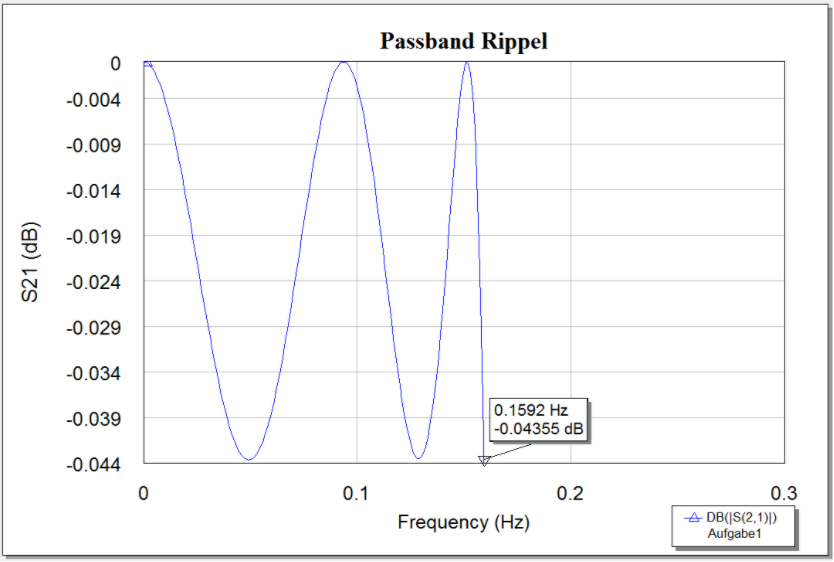
\includegraphics[width=\imagewidth]{images/Prototyp_Passbandrippel.png}
% 	\caption{Equirippel im Passband}
% 	\label{fig:Prototyp_Passbandrippel}
%\end{figure}
\begin{figure}[h!]
    \centering
    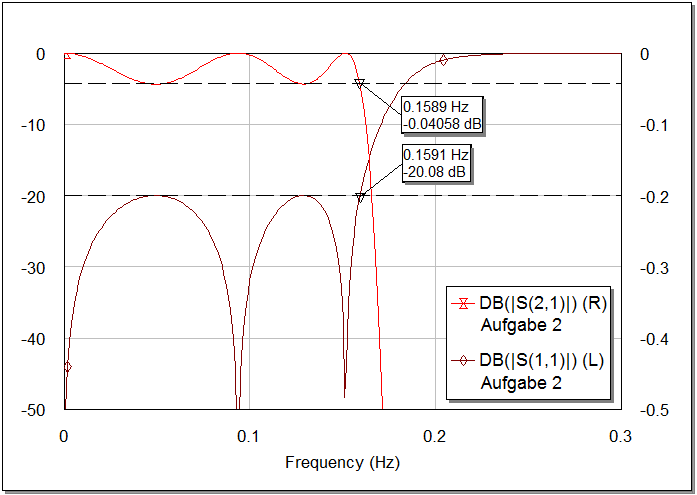
\includegraphics[width=\imagewidth]{images/graph-LC}
    \caption{}
    \label{fig:graph-LC}
\end{figure}

Ein verlustloses Filter lässt sich nicht nur mit der Einfgedämpfung S21 sondern auch mit der Reflexion S11 beschreiben, weil der folgende Zusammenhang gilt:

\begin{equation}
{|S11|}^2 + {|S21|}^2 = 1
\end{equation}

Somit kann die Reflexion im Passband mithilfe des Equirippels im Passband berechnet werden.

\begin{equation}
|S11| = \sqrt{1-{|Equirippel|}^2} = -20 dB
\end{equation}

Um das Resultat zu validieren, wurde die Reflexion S11 des Filter simuliert und in Abb. \ref{fig:graph-LC} dargestellt.

%\begin{figure}[h!]
%    \centering
% 	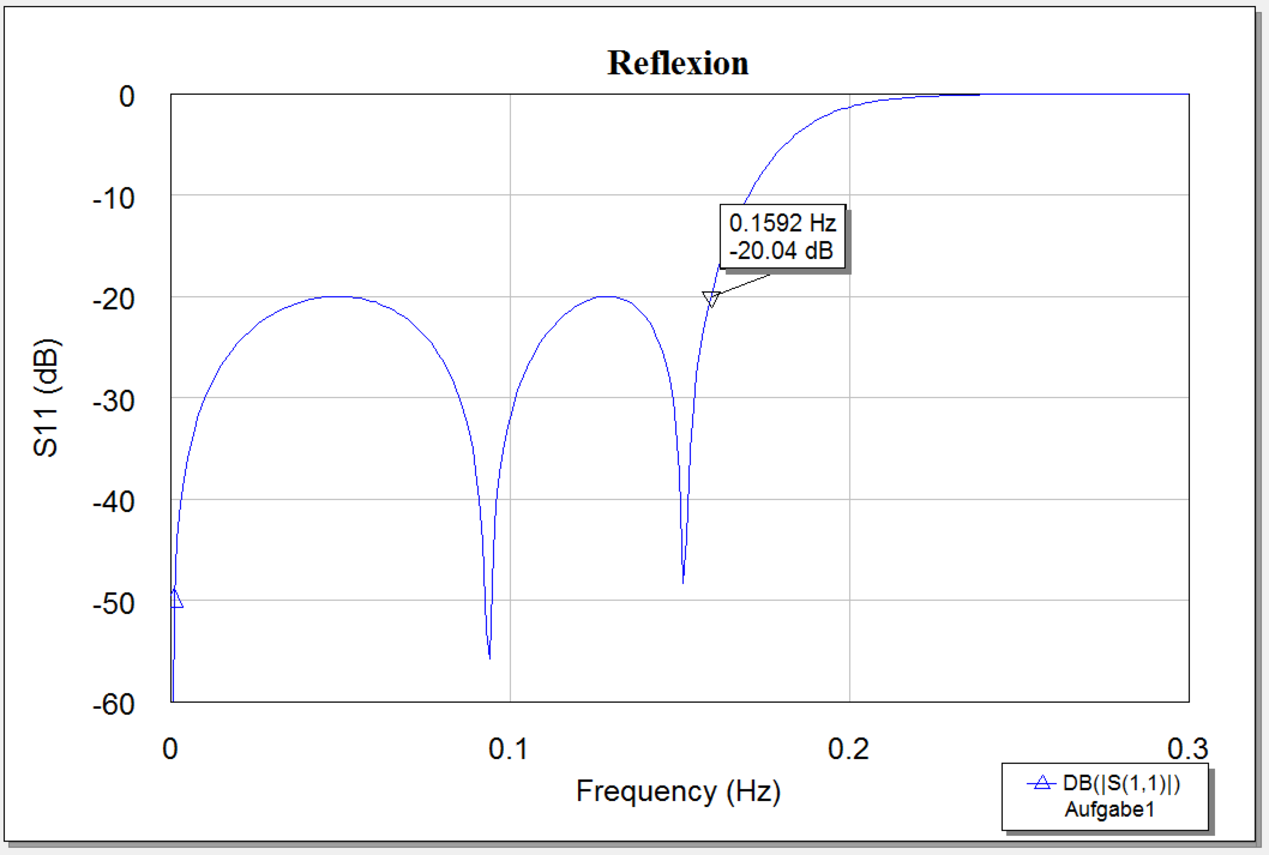
\includegraphics[width=\imagewidth]{images/Prototyp_Reflexion.png}
% 	\caption{Reflexion in Passband}
% 	\label{fig:Prototyp_Reflexion}
%\end{figure}

Es handelt sich beim zu realisierenden Stubfilter um ein Chebyshev Filter des Typ 1 mit folgenden Eigeschaften: 
\begin{mdframed}
    \begin{equation*} 
        \begin{array}{cllll} 
            f_C & = & 0.8 GHz \\ 
            f_\frac{\lambda}{4} & = & 2 GHz \\ 
            l & = & 37.5mm \\
            Equirippel (Passband) & = & -0.004355 dB \\
            Reflexion (Passband) & = & -20 dB \\
        \end{array} 
    \end{equation*} 
\end{mdframed}



